\newpage
\subsection{Сравнение тестов}\label{numerical_exp}

Кратко напомним тесты, которые будут сравниваться.
\begin{enumerate}
    \item $\varphi^{\text{Theta}}$ -- РНМН тест уровня 
    $\alpha=0.05$ проверки гипотезы
    $H^{\text{Theta}}: \theta=0$, где
     $\theta = \ln  \left(\dfrac{p_{001}p_{111}p_{010}p_{100}}{p_{011}p_{101}p_{000}p_{110}}\right)$.
    Поскольку из $X \ci Y \mid Z$ следует $\theta=0$, 
    то $\varphi^{\text{Theta}}$ также является несмещенным тестом уровня $\alpha=0.05$ проверки
    гипотезы $H:X \ci Y \mid Z$.
    \item $\varphi^{\text{Subsamples}}$ -- несмещенный тест уровня $\alpha=0.05$
    для проверки гипотезы $H: X \ci Y \mid Z$.
    Гипотеза $H$ отвергается, если РНМН-тестами уровня 
    $\gamma=1-\sqrt{1-\alpha}$
    отвергается хотя бы 
    одна гипотеза $H_z: \theta_z=0$, где
    $\theta_z = \ln\left(\dfrac{p_{00z}p_{11z}}{p_{01z}p_{10z}}\right)$.
    Напомним, что гипотеза $H_z: \theta_z=0$ проверяется по 
    по подвыборке из условного распределения $(X,Y)^T$ при условии $Z=z$.
    \item $\varphi^{\text{Partial}}$ -- точный тест уровня $\alpha=0.05$
    проверки гипотезы $H^{\text{Partial}}: \rho^{XY\cdot Z}~=~0$ в трехмерном нормальном распределении.
    % Если $\varphi^{\text{Partial}}$ -- также тест
    % уровня $\alpha=0.05$ для проверки гипотезы $\rho^{XY\cdot Z}=0$ в трехмерном распределении Бернулли, 
    % то $\varphi^{\text{Partial}}$ -- тест уровня $\alpha=0.05$ для проверки
    % гипотезы $h:X \ci Y \mid Z$ в трехмерном распределении Бернулли,
    % поскольку из $X \ci Y \mid Z$ следует $\rho^{XY\cdot Z}=0$.
\end{enumerate}

\begin{figure}[H]
    \centering
    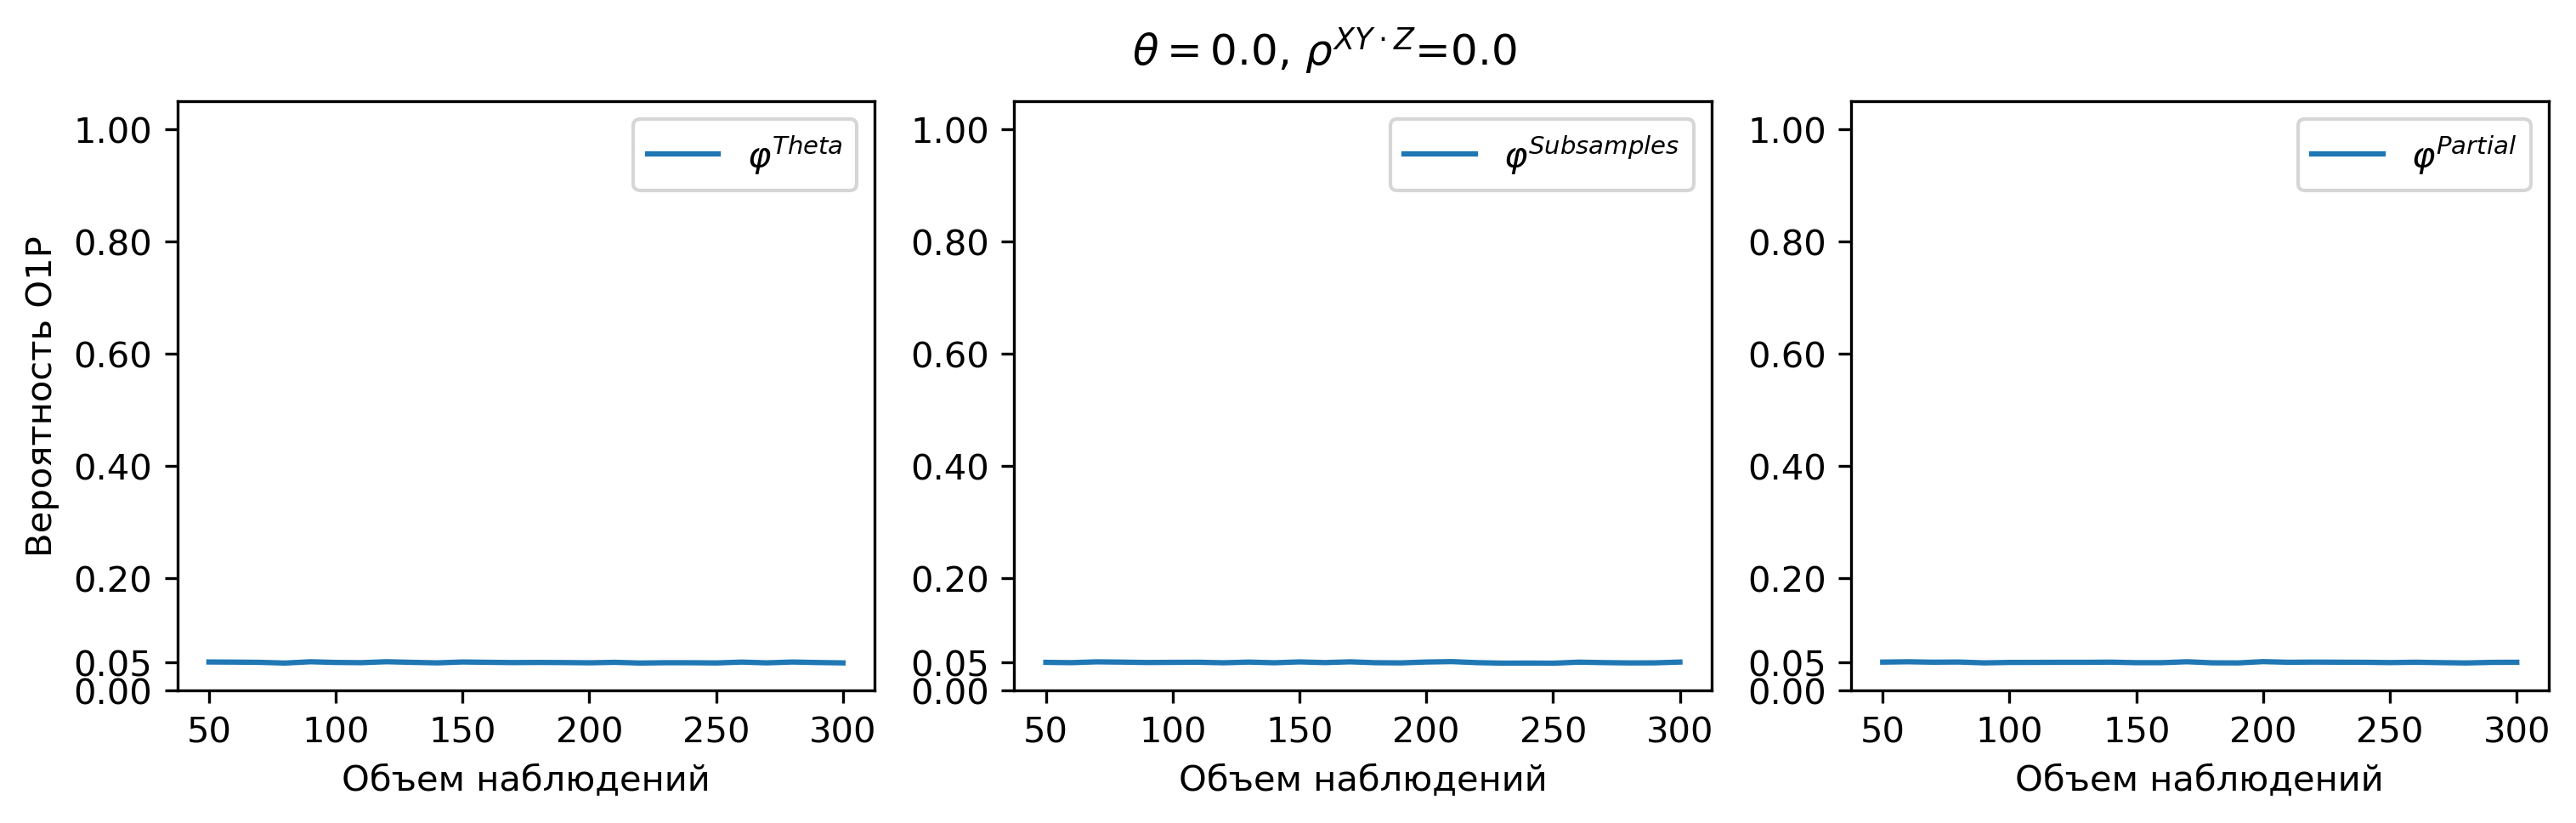
\includegraphics[scale=0.5]{images/graph1.png}
    \caption{Графики зависимости вероятности ошибки 1 рода (О1Р) от количества наблюдений,
     $p_{000}=0.125, p_{001}=0.125, p_{010}=0.125, p_{011}=0.125,
    p_{100}=0.125, p_{101}=0.125, p_{110}=0.125, p_{111}=0.125$. 
    Гипотеза $H: X \ci Y \mid Z$ верна.
    Вероятность оценивается по $10^5$ экспериментам.} \label{fig:1}
\end{figure}
    

\begin{figure}[H]
    \centering
    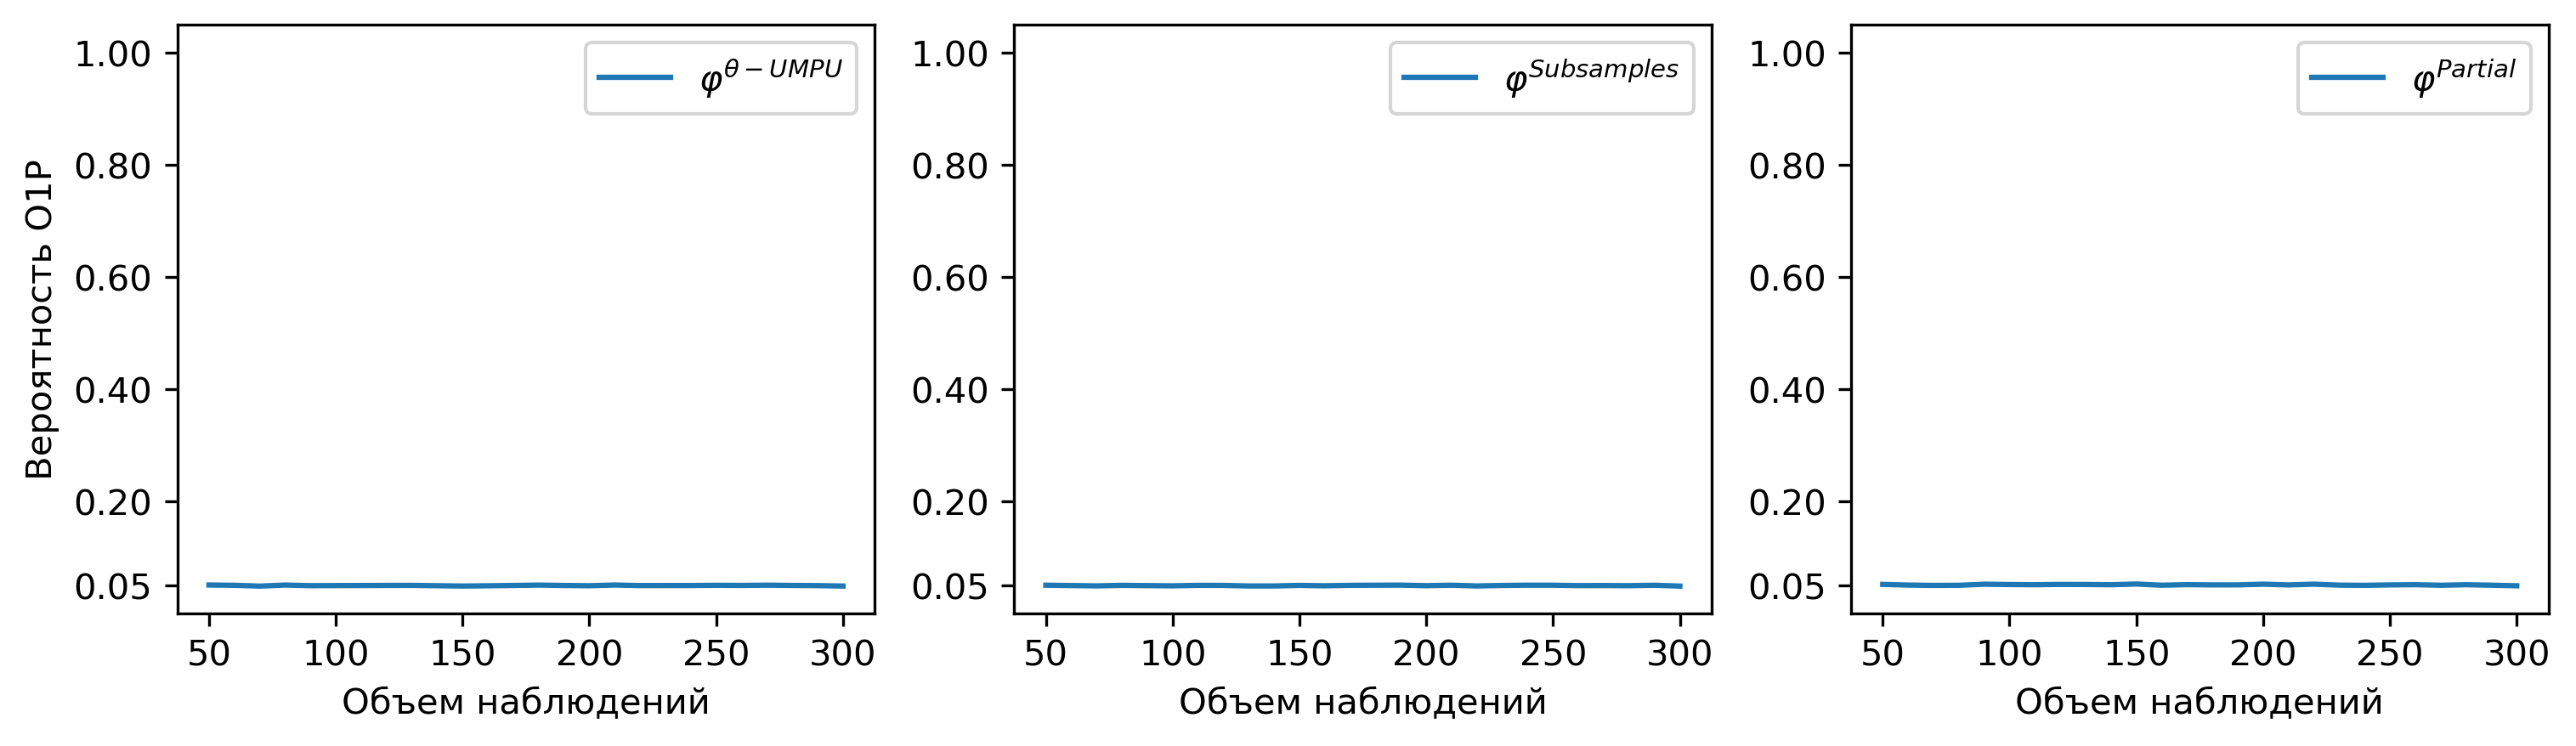
\includegraphics[scale=0.5]{images/graph2.png}
    \caption{Графики зависимости вероятности ошибки 1 рода (О1Р) от количества наблюдений,
    $p_{000}=0.15, p_{001}=0.1, p_{010}=0.3, p_{011}=0.1,
    p_{100}=0.05, p_{101}=0.1, p_{110}=0.1, p_{111}=0.1$. 
    Гипотеза $H: X \ci Y \mid Z$ верна.
    Вероятность оценивается по $10^5$ экспериментам.} \label{fig:2}
\end{figure}

\begin{figure}[H]
    \centering
    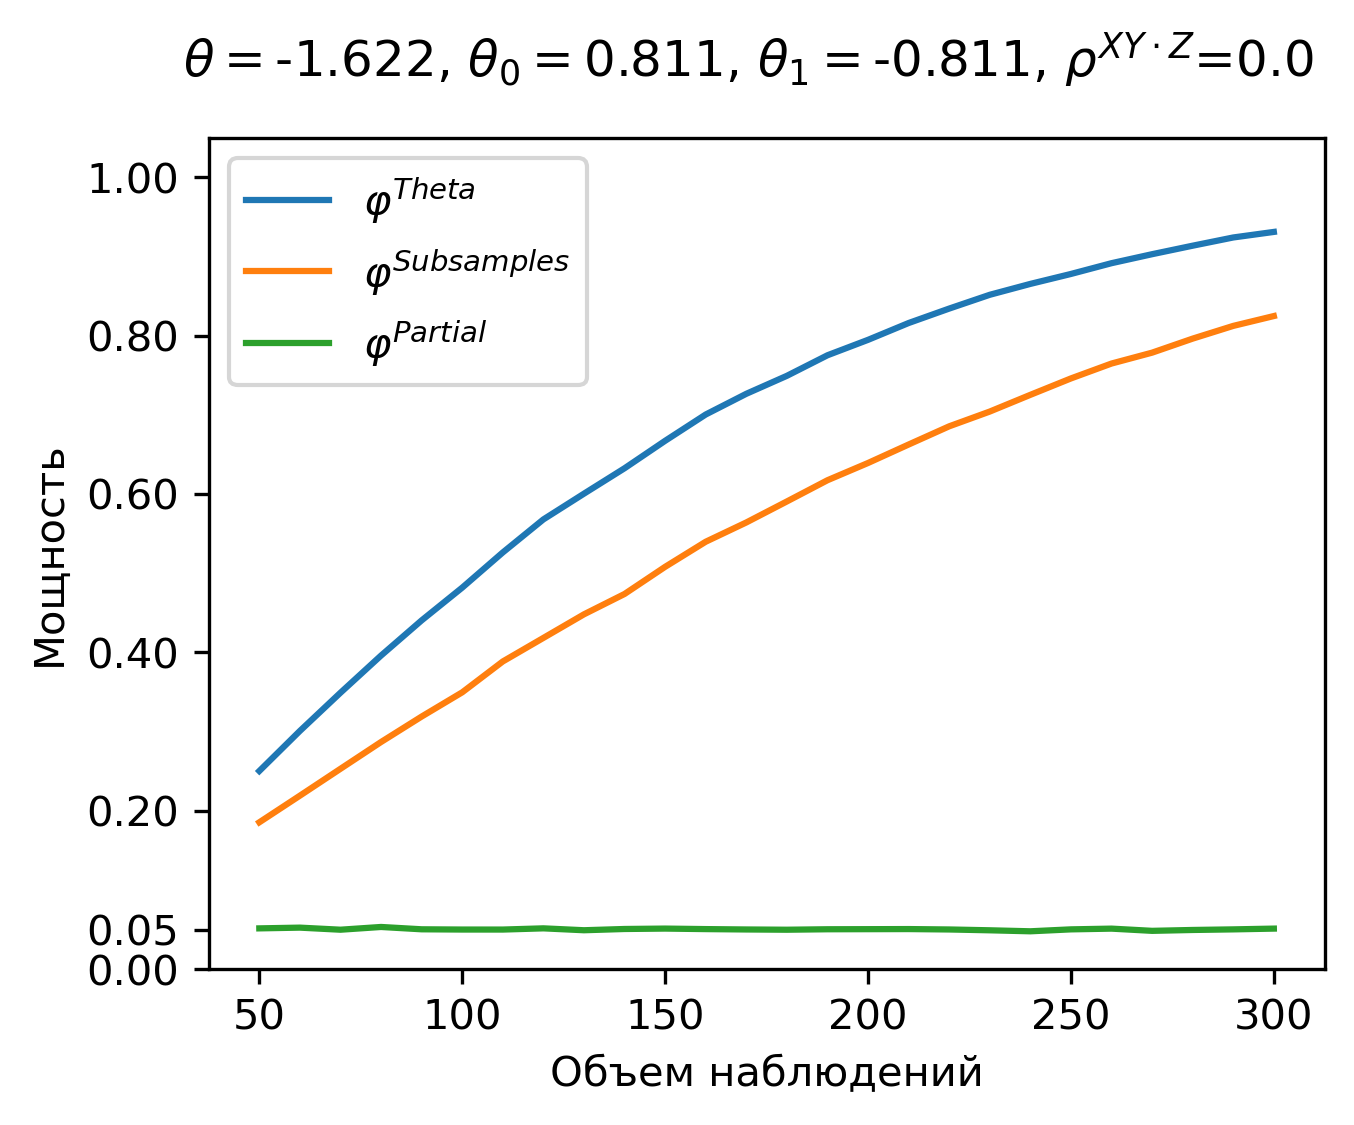
\includegraphics[scale=0.55]{images/graph4.png}
    \caption{График зависимости мощности от количества наблюдений,
    $p_{000}=0.15, p_{001}=0.1, 
    p_{010}=0.1, p_{011}=0.15,
    p_{100}=0.1, p_{101}=0.15, p_{110}=0.15, p_{111}=0.1$. 
    Гипотеза $H: X \ci Y \mid Z$ не верна, 
    однако верна гипотеза 
    $H^{\text{Partial}}: \rho^{XY\cdot Z}=0$.
    Мощность оценивается по $10^5$ экспериментам.} \label{fig:4}
\end{figure}

Из (\autoref{fig:1}) и (\autoref{fig:2}) видно, что 
для гипотезы $H: X \ci Y \mid Z$ тесты 
$\varphi^{\text{Theta}}$, $\varphi^{\text{Subsamples}}$, контролируют вероятность 
ошибки первого рода на уровне $\alpha=0.05$. Этот результат
полностью согласуется с теорией из \autoref{expon_form_section}, 
\autoref{twos}.

(\autoref{fig:1}), (\autoref{fig:2}), (\autoref{fig:4}) показывают,
что тест $\varphi^{\text{Partial}}$ контролирует вероятность
ошибки первого рода на уровне $\alpha=0.05$ для гипотезы
$H^\text{Partial}: \rho^{XY\cdot Z}=0$ в трехмерном
распределении Бернулли. Этот результат является неожиданным,
поскольку тест $\varphi^{\text{Partial}}$ теоретически обоснован
лишь для трехмерного нормального распределения.
Поскольку из $X \ci Y \mid Z$
следует $\rho^{XY\cdot Z}=0$, то тест $\varphi^{\text{Partial}}$ также
контролирует вероятность ошибки первого рода на уровне $\alpha=0.05$
и для гипотезы $H: X \ci Y \mid Z$, что показано на 
(\autoref{fig:1}), (\autoref{fig:2}).
Однако, стоит отметить,
что $\varphi^{\text{Partial}}$ проверяет необходимое условие 
условной независимости. Поэтому может возникнуть ситуация
как на (\autoref{fig:4}), когда гипотеза $H: X \ci Y \mid Z$ не верна, 
но тест $\varphi^{\text{Partial}}$ не распознает отклонение от условной независимости, поскольку
контролирует вероятность ошибки первого рода 
на уровне $\alpha=0.05$ для гипотезы $H^{\text{Partial}}: \rho^{XY\cdot Z}=0$.

\begin{figure}[H]
    \centering
    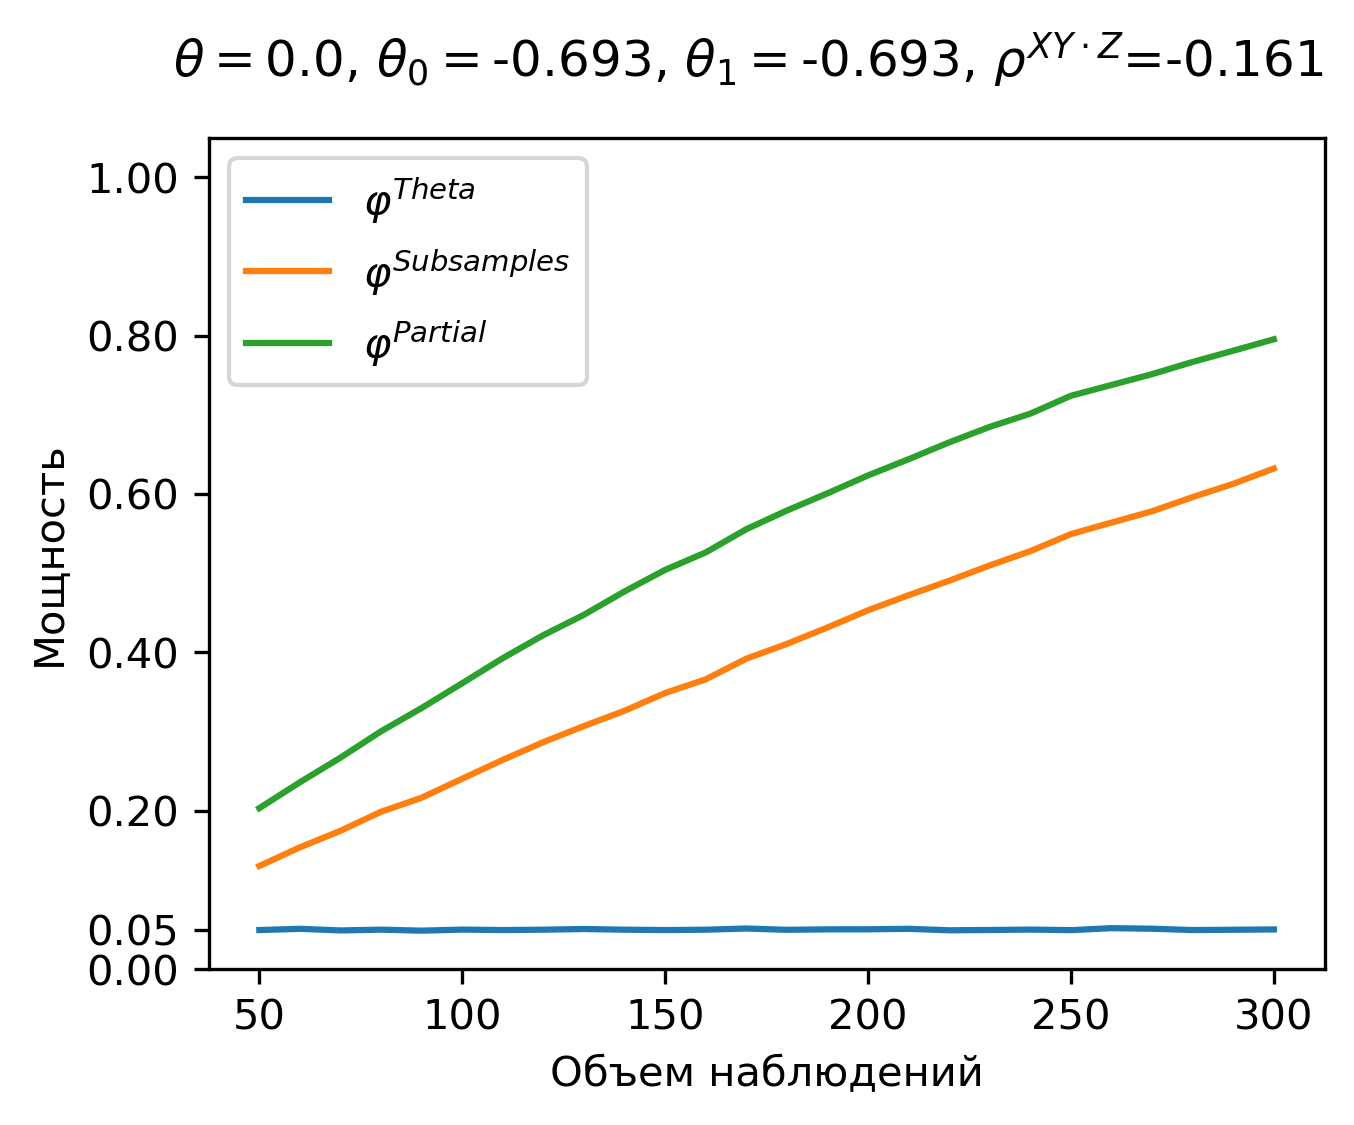
\includegraphics[scale=0.55]{images/graph5.png}
    \caption{График зависимости мощности от количества наблюдений,
    $p_{000}=0.15, p_{001}=0.05, 
    p_{010}=0.3, p_{011}=0.1,
    p_{100}=0.1, p_{101}=0.1, p_{110}=0.1, p_{111}=0.1$. 
    Гипотеза $H: X \ci Y \mid Z$ не верна, однако верны гипотезы $H^{\text{Theta}}: \theta=0$
    и $H^{\prime}: Y \ci Z \mid X$.
    Мощность оценивается по $10^5$ экспериментам.} \label{fig:5}
\end{figure}

Напомним, что тест 
$\varphi^{\text{Theta}}$ проверяет необходимое условие условной
независимости. Так на (\autoref{fig:5}) гипотеза 
$H: X \ci Y \mid Z$ не верна, 
но тест $\varphi^{\text{Theta}}$
не распознает отклонение от условной независимости и контролирует вероятность ошибки первого рода
на уровне $\alpha=0.05$ для гипотезы $H^{\text{Theta}}: \theta=0$.

Отметим, что $\varphi^{\text{Theta}}$ -- несмещенный тест уровня
$\alpha$ проверки гипотезы $H: X \ci Y \mid Z$.
Так как по \autoref{unbias} тест $\varphi^{\text{Subsamples}}$
является несмещенным тестом уровня $\alpha$ проверки гипотезы $H: X \ci Y \mid Z$, и 
на (\autoref{fig:5})
тест $\varphi^{\text{Subsamples}}$ мощнее теста $\varphi^{\text{Theta}}$,
то тест $\varphi^{\text{Theta}}$ не является РНМН тестом проверки 
гипотезы $H: X \ci Y \mid Z$, хотя является РНМН тестом
проверки гипотезы $H^{\text{Theta}}: \theta=0$.

\begin{figure}[H]
    \centering
    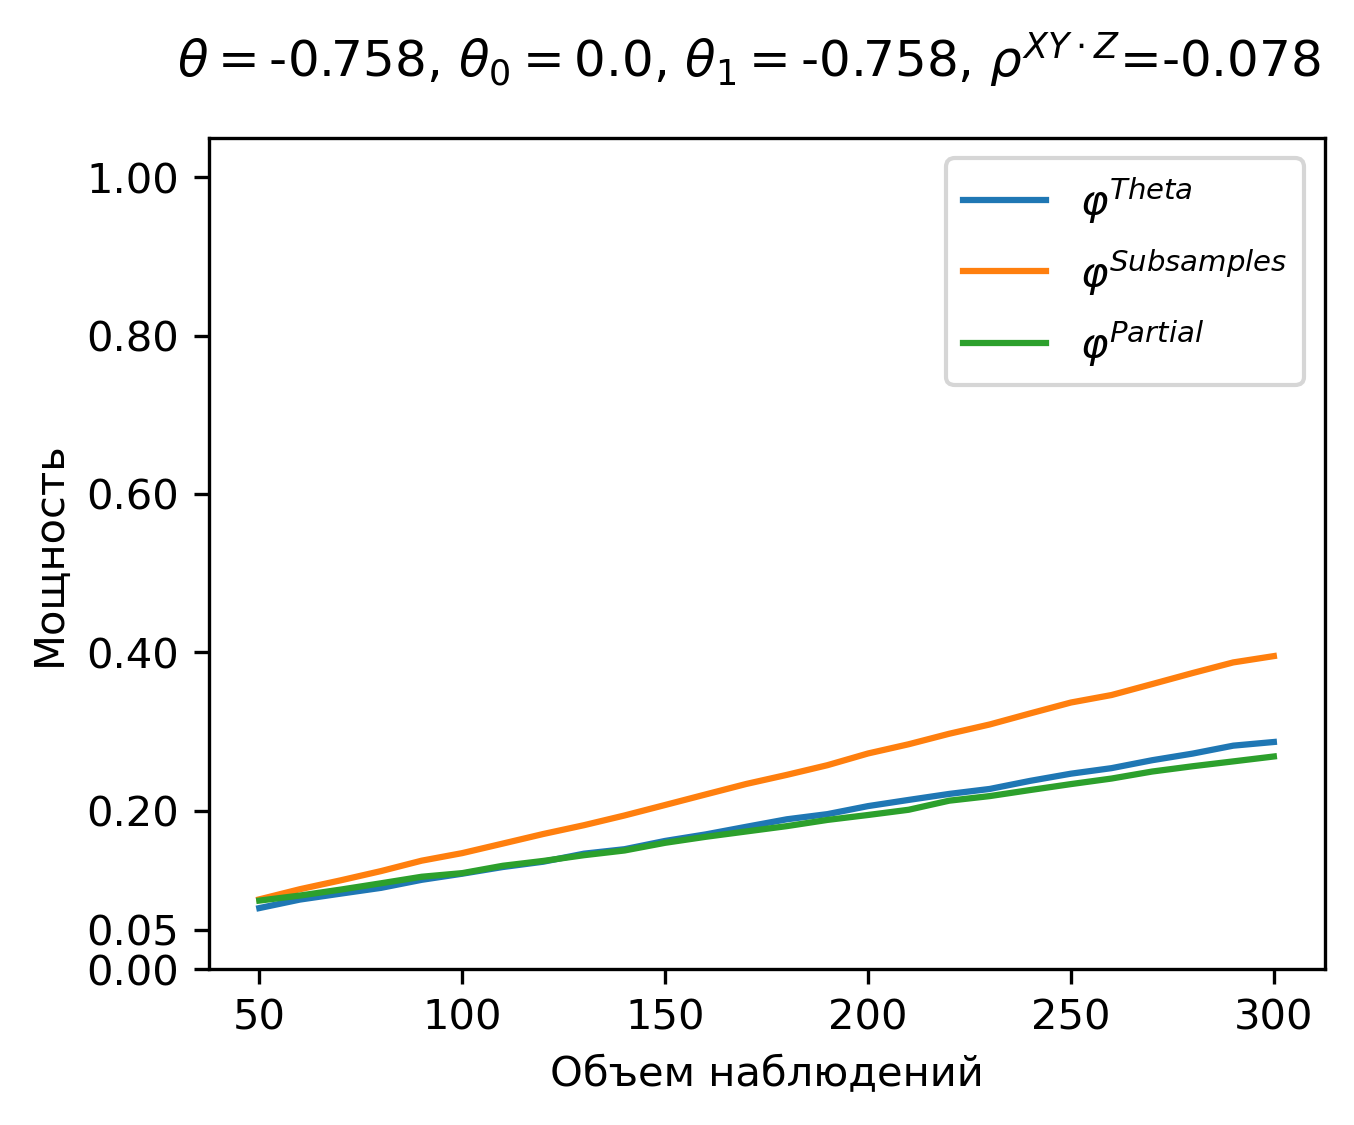
\includegraphics[scale=0.55]{images/graph3.png}
    \caption{График зависимости мощности от количества наблюдений,
    $p_{000}=0.15, p_{001}=0.06, 
    p_{010}=0.3, p_{011}=0.16,
    p_{100}=0.05, p_{101}=0.08, p_{110}=0.1, p_{111}=0.1$. 
    Гипотеза $H: X \ci Y \mid Z$ не верна, однако $X$ и $Y$ независимы
    при условии $Z=0$. 
    Мощность оценивается по $10^5$ экспериментам.}\label{fig:3}
\end{figure}

\begin{figure}[H]
    \centering
    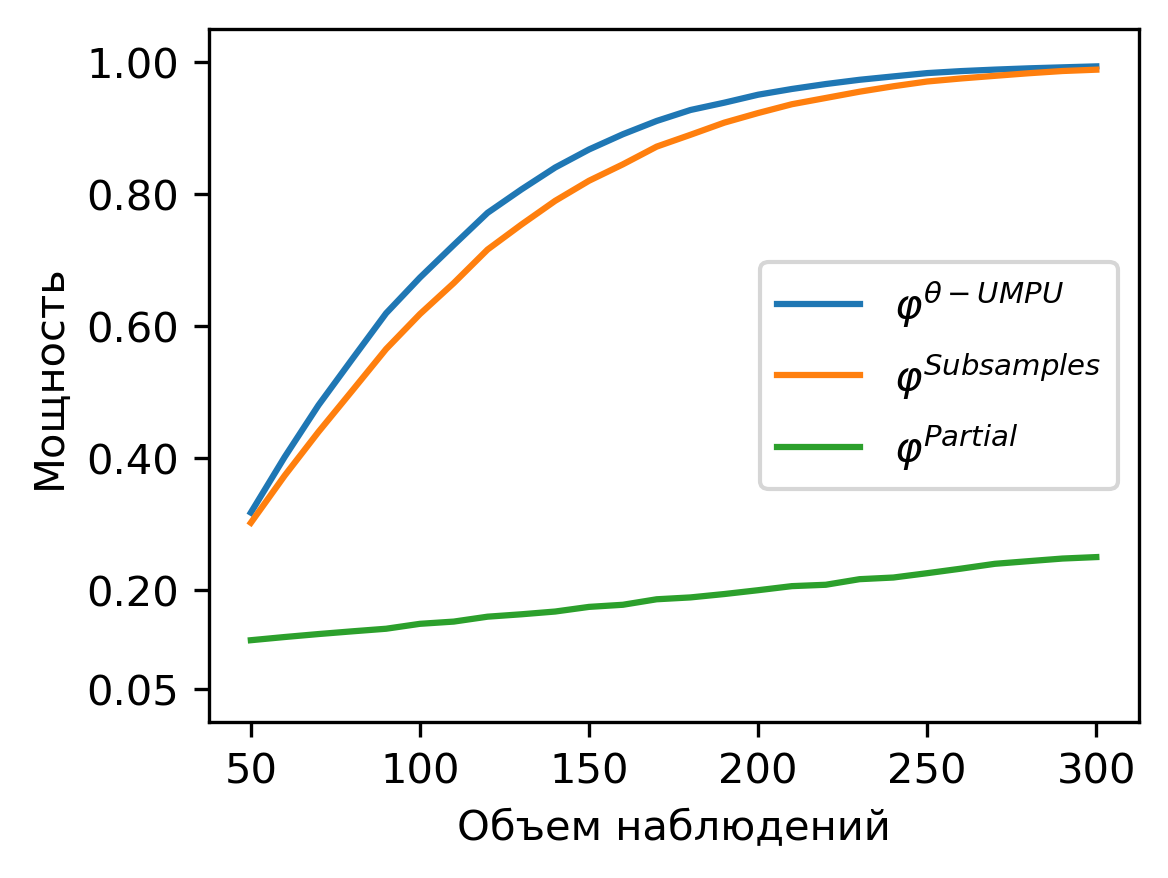
\includegraphics[scale=0.55]{images/graph6.png}
    \caption{График зависимости мощности от количества наблюдений,
    $p_{000}=0.03, p_{001}=0.1, 
    p_{010}=0.04, p_{011}=0.08,
    p_{100}=0.3, p_{101}=0.1, p_{110}=0.07, p_{111}=0.28$. 
    Гипотеза $H: X \ci Y \mid Z$ не верна.
    Мощность оценивается по $10^5$ экспериментам.} \label{fig:6}
\end{figure}

\begin{figure}[H]
    \centering
    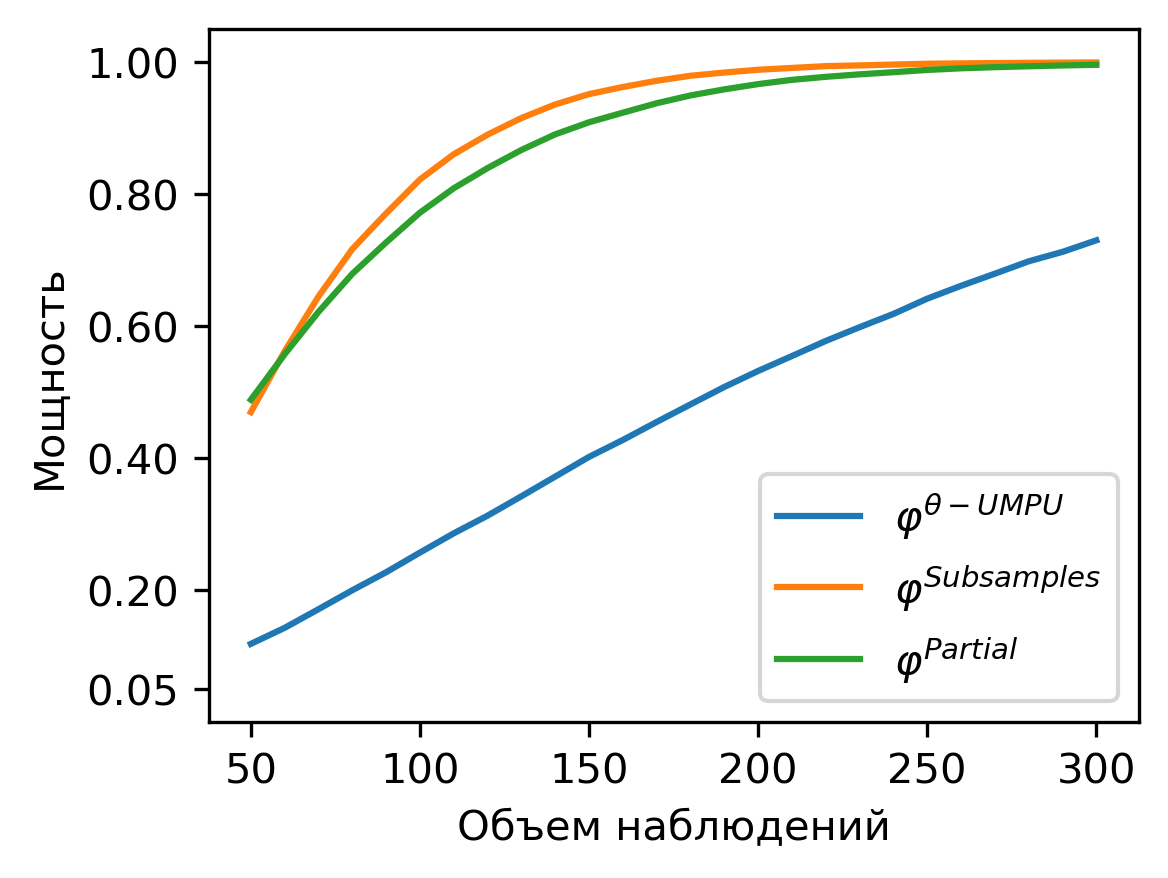
\includegraphics[scale=0.55]{images/graph7.png}
    \caption{График зависимости мощности от количества наблюдений,
    $p_{000}=0.21, p_{001}=0.12, 
    p_{010}=0.04, p_{011}=0.34,
    p_{100}=0.1, p_{101}=0.12, p_{110}=0.02, p_{111}=0.05$. 
    Гипотеза $H: X \ci Y \mid Z$ не верна.
    Мощность оценивается по $10^5$ экспериментам.} \label{fig:7}
\end{figure}

(\autoref{fig:4}), (\autoref{fig:5}), 
(\autoref{fig:3}), (\autoref{fig:6}), (\autoref{fig:7})
показывают, что, вообще говоря, рассматриваемые тесты нельзя упорядочить по мощности.
Кроме того, несмещенные тесты $\varphi^{\text{Subsamples}}$
и $\varphi^{\text{Theta}}$ уровня $\alpha$ проверки
гипотезы $H: X \ci Y \mid Z$ также нельзя упорядочить по мощности.
Поэтому вопрос построения РНМН теста проверки гипотезы 
$H: X \ci Y \mid Z$ остается открытым. 


% Одним из возможных отклонений от условной независимости является случай,
% когда $X$ и $Y$ независимы при условии $Z=0$, но зависимы при условии $Z=1$.
% Пример (\autoref{fig:3}) показывает, ...

% Показательным является пример с (\autoref{fig:6}). Тесты 
% $\varphi^{\text{Theta}}$ и $\varphi^{\text{Subsamples}}$ при $n=300$
% наблюдениях имеют мощность, близкую к $1$. В то время как мощность
% теста $\varphi^{\text{Partial}}$ приблизительно равна $0.25$. Это происходит потому, что
% в данном примере значение $\rho^{XY\cdot Z}=0.068$ близко к нулю.


% Еще интересен пример с (\autoref{fig:7}). 
% При $n=300$ наблюдениях мощность тестов
% $\varphi^{\text{Subsamples}}$, $\varphi^{\text{Partial}}$ близка к $1$,
% в то время как мощность теста $\varphi^{\text{Theta}}$ примерно равна $0.73$.

% В данном разделе были изложены результаты численных экспериментов с тестами
% $\varphi^{\text{Theta}}$, $\varphi^{\text{Subsamples}}$, 
% $\varphi^{\text{Partial}}$ при $\alpha=0.05$. На 
% (\autoref{fig:1}) и (\autoref{fig:2}) показано, что 
% при истинности гипотезы  
% $h: X \ci Y \mid Z$ эти тесты контролируют вероятность ошибки первого рода
% на уровне $\alpha=0.05$. 
% Однако, за счет того, что тесты 
% $\varphi^{\text{Subsamples}}$ и
% $\varphi^{\text{Partial}}$ проверяют более широкие гипотезы,
% возникают ситуации как на 
%  (\autoref{fig:4}) и (\autoref{fig:5}), когда гипотеза $h: X \ci Y \mid Z$
% не верна и мощность теста равна $0.05$ при любом объеме наблюдений.
% Особым образом можно выделить тест $\varphi^{\text{Subsamples}}$.
% На всех графиках $\varphi^{\text{Subsamples}}$ либо лучший по мощности,
% либо незначительно уступает лучшему по мощности тесту.
